\chapter{Evaluation}

This evaluation centers on a realistic editing scenario, where we assume that the user has a specific set of code modifications they wish to implement. Our primary objective is to determine how effectively the proposed approach replicates human behavior and intent during these edits. By examining how closely the system’s actions align with typical manual editing patterns, we gain insight into its potential to streamline development workflows and reduce the need for extensive manual intervention.

\section{Dataset}

We construct a dataset of five programming languages (Python, Go, Java, JavaScript, and TypeScript), which consists of 689 most-starred repositories from GitHub,
with 38,197 commits. Dataset statistics are shown in Table \ref{tab:dataset-stats}.

\begin{table}[htbp]
\centering
\begin{tabular}{lcccc}
\hline
\textbf{Language} 
  & \textbf{\# Repositories} 
  & \textbf{\# Commits} 
  & \textbf{\# Edits} \\
\hline
\textbf{Python}      
  & 125   & 8148  
  & 51288 \\

\textbf{Go}          
  & 165   & 7031    
  & 46436 \\

\textbf{Java}        
  & 107   & 13539 
  & 96903 \\

\textbf{JavaScript}  
  & 124   & 2610      
  & 15833 \\

\textbf{TypeScript}  
  & 168  & 7319     
  & 51597\\
\hline
\textbf{Total}       
  & 689 & 38197
  & 257654 \\
\hline
\end{tabular}
\caption{Dataset statistics for each language.}
\label{tab:dataset-stats}
\end{table}

We choose code commits from popular code repositories on GitHub, each of which has a set of edits and a code commit message. The challenges lie in how to construct a dataset which can be representative to real-world software development tasks,  especially when the number of code windows is sufficiently large. In this work, instead of randomly sampling the code windows in a project, we propose a sampling technique for code windows with representative diversity.

\begin{figure}[htbp]
\centering
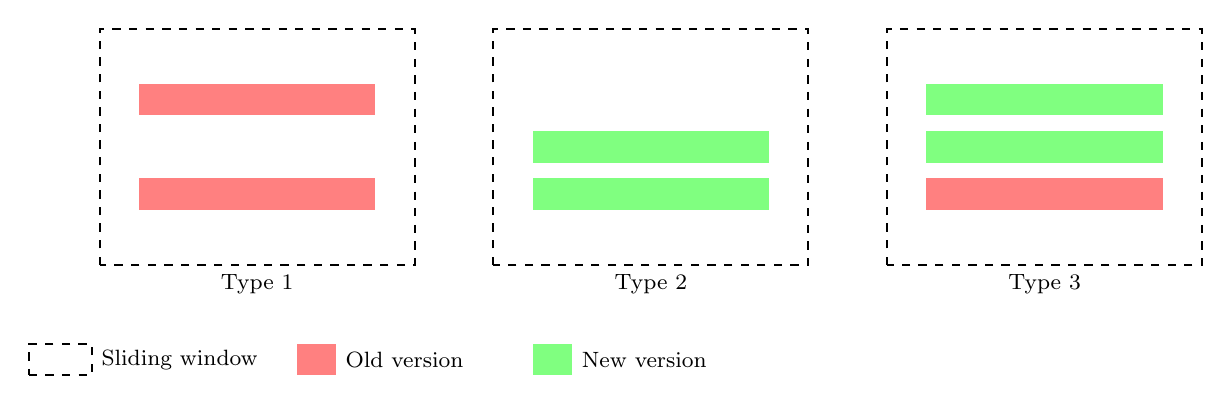
\begin{tikzpicture}[font=\footnotesize]
%--- TYPE 1 ---
% Make the rectangle wider: (0,0) rectangle (3,2) -> 3 units wide
\draw[dashed, thick] (1.5,0) rectangle (5.5,3);
\node[below] at (3.5,0) {Type 1};
% Widen the red bars accordingly
\fill[red!50] (2,2.3) rectangle (5,1.9);
\fill[red!50] (2,1.1) rectangle (5,0.7);

%--- TYPE 2 ---
% Shift this window to the right and make it also 3 units wide
\draw[dashed, thick] (6.5,0) rectangle (10.5,3);
\node[below] at (8.5,0) {Type 2};
\fill[green!50] (7,1.7) rectangle (10,1.3);
\fill[green!50] (7,1.1) rectangle (10,0.7);

%--- TYPE 3 ---
% Shift further and make it 3 units wide
\draw[dashed, thick] (11.5,0) rectangle (15.5,3);
\node[below] at (13.5,0) {Type 3};
% Top "new version" bar (green)
\fill[green!50] (12,2.3) rectangle (15,1.9);
\fill[green!50] (12,1.7) rectangle (15,1.3);
% Bottom "old version" bar (red)
\fill[red!50]   (12,1.1) rectangle (15,0.7);

%--- LEGEND (optional) ---
\node[draw, dashed, thick, minimum width=0.8cm, minimum height=0.4cm]
      at (1,-1.2) {};
\node[right] at (1.4,-1.2) {Sliding window};

\fill[red!50] (4,-1.4) rectangle (4.5,-1);
\node[right] at (4.5,-1.2) {Old version};

\fill[green!50] (7,-1.4) rectangle (7.5,-1);
\node[right] at (7.5,-1.2) {New version};
\end{tikzpicture}
\caption{Sampling strategy of sliding window with real-world edit dynamic}
\label{fig:dataset}
\end{figure}

We sample three types of code windows from a commit, as shown in Figure \ref{fig:dataset}: 

\begin{itemize}
    \item Type 1: A code window with 1 or more edits that involve only deletion, each edit may be complete or partial, as shown in red in the first window type.
    \item Type 2: A code window with 1 or more edits that involve only addition, each edit may be complete or partial, as shown in green in the second window type.
    \item Type 3: A code window containing a mixed of different types of edits, notably addition, deletion and modification as shown in the third window type.
\end{itemize}

In the dataset, the occurred changes in the code window are informative to refrain from unnecessary recommendations on those areas. We sample the above types with a ratio of 1:1:3. We then further adopt $Llama-3-8B-Instruct$ to filter out commits with messages containing vague instructions or multiple intentions, as these contents hinder the model from establishing proper semantic connection between natural language and code editing. The passed commits have their messages refined for brevity and clarity (e.g., removing pull request IDs or committer emails). Our manual check shows that refined commit messages are more natural as edit descriptions, with redundancy removed.

As a result, the three types of sliding windows can reflect the distribution of real-world editing scenarios in terms of edit label position within the window, edit label quantity and edit dynamics.

\section{Recovering Edit Process}

Following the methodology outlined in Section \ref{sec:por}, our goal is to reconstruct the edit sequence of each commit. Once the pairwise dependencies of edits within a commit have been identified, we introduce a framework for deriving \emph{constrained orderings} of nodes in a Directed Acyclic Graph (DAG). We formalize the notion of topological sorts subject to group-based constraints, as well as a depth-first traversal variant that similarly respects user-defined grouping. We provide detailed algorithms that demonstrate how to compute every possible valid ordering.

\subsection{Preliminaries and Notations}

In some scenarios, \emph{additional grouping constraints} are introduced; these constraints require the algorithm to consider certain subsets of nodes (groups) in a particular sequence. We call the resulting orderings \emph{constrained orderings}.

Let $G = (V, E)$ be a directed acyclic graph (DAG), where
\begin{itemize}
    \item $V = \{1,2,\ldots,n\}$ is the set of $n$ nodes.
    \item $E \subseteq V \times V$ is the set of directed edges.
\end{itemize}
An edge $(u,v) \in E$ means $u$ must appear before $v$ in any valid ordering.  
We denote the \emph{indegree} of a node $v \in V$ by $\text{indegree}(v)$, the number of incoming edges to $v$.

\subsection{Constrained Grouping}
We consider a partition (or covering) of the node set $V$ into $k$ groups: 
\[
  \mathcal{G} = \{G_1, G_2, \dots, G_k\} 
  \quad \text{where} \quad
  \bigcup_{i=1}^{k} G_i = V, 
\]
and each $G_i \subseteq V$. We assume a user-specified \emph{ordering} on these groups, denoted by \\ $(G_{\pi(1)}, G_{\pi(2)}, \dots, G_{\pi(k)})$, where $\pi$ is a permutation of $\{1,2,\ldots,k\}$. 

The overarching idea is to \emph{respect group order} when constructing a node ordering of $V$: we do not move on to $G_{\pi(i+1)}$ before we exhaust possible nodes in $G_{\pi(i)}$, subject to each node's DAG-based indegree conditions.

\subsection{Topological Sorts with Group Constraints}
\label{sec:topo-group}
\begin{algorithm}[H]
\caption{Topological Sort by Group Order}
\label{alg:topological-sorts-by-group}
\begin{algorithmic}[1]
\Require DAG $G=(V,E)$, \text{indegree} map $\text{indegree}(\cdot)$, group order $(G_1, G_2, \dots, G_k)$
\Ensure All constrained topological orderings of $V$

\State Initialize $\text{visited} \gets \varnothing$, $\text{path} \gets []$

\Function{Backtrack}{path, i}
    \If{$|\text{path}| = |V|$}
        \State \textbf{yield} \text{path} \text{ as a valid ordering}
        \State \Return
    \EndIf
    \State $\text{current\_group} \gets G_i$
    \For{\textbf{each} $n$ in $\text{current\_group}$}
        \If{$n \notin \text{visited}$ \textbf{and} $\text{indegree}(n) = 0$}
            \State $\text{visited} \gets \text{visited} \cup \{n\}$
            \State $\text{path}.\text{append}(n)$
            \For{\textbf{each} neighbor $w$ of $n$ in $G$}
                \State $\text{indegree}(w) \gets \text{indegree}(w) - 1$
            \EndFor
            \State \Call{Backtrack}{path, i}
            \For{\textbf{each} neighbor $w$ of $n$}
                \State $\text{indegree}(w) \gets \text{indegree}(w) + 1$
            \EndFor
            \State $\text{path}.\text{pop}()$
            \State $\text{visited} \gets \text{visited} \setminus \{n\}$
        \EndIf
    \EndFor
    \If{$i + 1 < k$}
        \State \Call{Backtrack}{path, i + 1}
    \EndIf
\EndFunction

\State \Call{Backtrack}{[], 0}

\end{algorithmic}
\end{algorithm}

The procedure in Algorithm~\ref{alg:topological-sorts-by-group} 
explores all possible ways to pick a node from the current group $G_i$ whenever that node has $\text{indegree}(n) = 0$. As soon as a node $n$ is chosen, it is appended to the path, and the indegree of its neighbors is decreased. We recursively proceed until the entire node set is exhausted or move on to the next group. Each valid path upon reaching full length is a \emph{constrained topological ordering}.

\subsection{Finding Connected Components (Undirected View)}
Although our graph is a DAG, for some applications, we also need to consider the \emph{undirected} version of $G$, denoted $G^{u} = (V, E^{u})$, where $E^{u} = \{\{u,v\} \mid (u,v)\in E \lor (v,u)\in E\}$. A standard Depth-First Search (DFS) on $G^{u}$ identifies connected components.
\begin{algorithm}[H]
\caption{Connected Components in Undirected Graph}
\label{alg:connected-components}
\begin{algorithmic}[1]
\Require Node set $V$, edge set $E$ (directed; treat as undirected here)
\Ensure All connected components $\{C_1, C_2, \ldots\}$

\State Construct $G^{u} = (V, E^{u})$ where $E^{u}$ is the undirected version of $E$
\State $\text{visited} \gets \varnothing$

\Function{DFS}{u, component}
    \State $\text{visited} \gets \text{visited} \cup \{u\}$
    \State $\text{component}.\text{append}(u)$
    \For{\textbf{each} neighbor $w$ of $u$ in $G^{u}$}
        \If{$w \notin \text{visited}$}
            \State \Call{DFS}{w, component}
        \EndIf
    \EndFor
\EndFunction

\For{\textbf{each} node $v$ in $V$}
    \If{$v \notin \text{visited}$}
        \State $\text{component} \gets []$
        \State \Call{DFS}{v, component}
        \State \textbf{yield} $\text{component}$
    \EndIf
\EndFor
\end{algorithmic}
\end{algorithm}


\subsection{Depth-First Traversal by Group}
\label{sec:dfs-group}
In some cases, rather than enforcing a globally minimal node first policy (as in topological sort), one may wish to run a DFS while still \emph{respecting group constraints}. 
\begin{algorithm}[H]
\caption{Depth-First Traversal by Group}
\label{alg:depth-first-traversal-by-group}
\begin{algorithmic}[1]

\Require DAG \(G = (V,E)\), \(\text{indegree}\) map \(\text{indegree}(\cdot)\), group order \((G_1, \ldots, G_k)\)
\Ensure Constrained depth-first traversals of \(V\)

\Function{FindStartingNodes}{G\_i}
    \State \Return \(\{\,v \in G\_i \mid \text{indegree}(v) = 0\,\}\)
\EndFunction

\Function{DFSCompleteTraversal}{s, G\_i, visited, traversal}
    \State stack \(\gets [\,s\,]\)
    \While{stack is not empty}
        \State \(n \gets \text{stack.pop}()\)
        \If{\(n \notin visited\)}
            \State \(visited \gets visited \cup \{n\}\)
            \State \(\text{traversal.append}(n)\)
            \For{\textbf{each} neighbor \(w\) of \(n\) in \(G\)}
                \If{\(w \notin visited\)}
                    \State \(\text{stack.push}(w)\)
                \EndIf
            \EndFor
        \EndIf
    \EndWhile

    \For{\(m \in \Call{FindStartingNodes}{G\_i}\)}
        \If{\(m \notin visited\)}
            \State \Call{DFSCompleteTraversal}{m, G\_i, visited, traversal}
        \EndIf
    \EndFor
\EndFunction

\State \(S \gets \bigl[\Call{FindStartingNodes}{G_1},\dots,\Call{FindStartingNodes}{G_k}\bigr]\)
\Comment{Set of starting nodes per group}

\For{\((s_1,\dots,s_k) \in \prod_{i=1}^k S_i\)}
    \State \(visited \gets \varnothing\)
    \State \(traversal \gets [\,]\)
    \For{\(i \gets 1 \text{ to } k\)}
        \If{\(s_i \notin visited\)}
            \State \Call{DFSCompleteTraversal}{s_i, G_i, visited, traversal}
        \EndIf
    \EndFor
    \State \textbf{yield} \(traversal\)
\EndFor

\end{algorithmic}
\end{algorithm}


Algorithm~\ref{alg:depth-first-traversal-by-group} shows how we generate all possible DFS-based traversals while forcing the sequence of groups. We collect possible \emph{starting nodes} in each group based on $\text{indegree}$ conditions. The \textbf{product} of these sets of starting nodes yields different ways to initiate a DFS in each group. Then, for each combination of starting nodes, we do a full DFS while ensuring that if further valid starting nodes exist in $G_i$, they are explored before switching to the next group $G_{i+1}$.

\subsection{Enumerating All Constrained Sorts for Every Group Ordering}
We can further iterate over every \emph{permutation} of the groups to find all distinct ways the groups may be arranged:
\[
  \text{Permutations of } (G_1, G_2, \dots, G_k) \;=\; \{\,(G_{\pi(1)}, \dots, G_{\pi(k)}) \;|\; \pi \text{ is any permutation of } \{1,\dots,k\}\}.
\]
\begin{algorithm}[H]
\caption{Constrained Sorts for All Group Orders}
\label{alg:constrained-sorts-all-group-orders}
\begin{algorithmic}[1]

\Require \(G = (V,E)\), \(\text{indegree}\) map \(\text{indegree}(\cdot)\), set of nodes \(V\),
        all permutations \(\{\pi_1,\dots,\pi_M\}\) of group partitions,
        boolean \(\text{topo}\) to switch method
\Ensure All constrained node orderings according to each permutation

\For{\textbf{each} permutation \(\pi_j\)}
    \If{\(\text{topo} = \text{True}\)}
        \State \textbf{yield all} \Call{TopologicalSortsByGroup}{\(G, \text{indegree}, V, \pi_j\)}
    \Else
        \State \textbf{yield all} \Call{DepthFirstTraversalByGroup}{\(G, \text{indegree}, \pi_j\)}
    \EndIf
\EndFor

\end{algorithmic}
\end{algorithm}

We have introduced a framework for deriving \emph{constrained orderings} of nodes in a directed acyclic graph. The two major approaches demonstrated are:
\begin{itemize}
    \item A group-constrained \emph{topological sort}, ensuring that nodes are chosen in zero-indegree fashion \emph{within} each group before moving on.
    \item A group-constrained \emph{DFS} approach, enumerating all ways to initiate a DFS for each group, respecting partial orders.
\end{itemize}
By iterating over all permutations of groups, we obtain the full set of valid orderings. This approach can be specialized for tasks such as constrained scheduling, compilation ordering, or phased execution where partial orders must be respected, but some steps are grouped logically.

\section{Evaluation Workflow}
Let $C = \{\,C^{(1)}, C^{(2)}, \dots, C^{(m)}\} $ be the set of all valid orderings of the ground-truth changes. Given a predicted sequence, $P$, we first check whether $P$ exactly matches any $C^{(i)} \in C$.

If there exists an $i$ such that $P = C^{(i)}$, we consider $P$ a perfect match and assign zero cost.

Otherwise, we compute the minimum number of swaps needed to transform $P$ into each $C^{(i)}$, and select 
$\min_{1 \leq i \leq m} \bigl(\mathrm{MinSwaps}(P, C^{(i)})\bigr)$ as the distance metric. Here, $\mathrm{MinSwaps}(\cdot,\cdot)$ measures the minimum swaps required to reorder one permutation into another (assuming both contain the same elements.


\begin{algorithm}[H]
\caption{Minimum Swaps Between Two Permutations}
\label{alg:min-swaps}
\begin{algorithmic}[1]
\Require Two permutations $p$ and $q$ of length $n$
\Ensure The minimum number of swaps needed to transform $p$ into $q$

\Statex

\State \(\textit{inv} \gets \text{array of length } n\)
\For{\(i \gets 1 \text{ to } n\)}
    \State \(\textit{inv}[\,p[i]\,] \gets i\)
\EndFor

\State \(r \gets \text{array of length } n\)
\For{\(i \gets 1 \text{ to } n\)}
    \State \(r[i] \gets \textit{inv}[\,q[i]\,]\)
\EndFor

\State \(\textit{visited} \gets \text{boolean array of length } n\text{, all } \textbf{false}\)
\State \(\textit{countCycles} \gets 0\)

\For{\(i \gets 1 \text{ to } n\)}
    \If{\(\neg \textit{visited}[i]\)}
        \State \(\textit{countCycles} \gets \textit{countCycles} + 1\)
        \State \(j \gets i\)
        \While{\(\neg \textit{visited}[j]\)}
            \State \(\textit{visited}[j] \gets \textbf{true}\)
            \State \(j \gets r[j]\)
        \EndWhile
    \EndIf
\EndFor

\State \(\textit{minSwaps} \gets n - \textit{countCycles}\)
\State \Return \(\textit{minSwaps}\)

\end{algorithmic}
\end{algorithm}

The evaluation results for Python repositories can be seen below: 

\begin{table}[h!]
\centering
\caption{Comparison of Various Programming Languages}
\label{tab:language-comparison}
\begin{tabular}{@{}lrrrrrrr@{}}
\toprule
\textbf{Language} & \textbf{\# Commits} & \textbf{Perfect Matches} & \textbf{Min Swaps} & \textbf{Max Swaps} & \textbf{Avg} & \textbf{Median} & \textbf{Std Dev} \\ 
\midrule
TypeScript & 103 & 22 & 2  & 26 & 10.2 & 9  & 4.1 \\
Python     &  89 & 19 & 1  & 38 & 12.4 & 11 & 5.2 \\
JavaScript &  67 & 13 & 2  & 16 &  7.8 & 7  & 3.5 \\
Go (Golang)&  56 &  9 & 0  & 20 &  8.9 & 7  & 4.3 \\
Java       & 115 & 27 & 3  & 34 & 14.1 & 13 & 6.0 \\
\bottomrule
\end{tabular}
\end{table}
